\providecommand{\main}{../../../..}
\documentclass[\main/dresen_thesis.tex]{subfiles}
\begin{document}
  \label{sec:colloidalCrystals:layers:pnr}

  \begin{figure}[tb]
    \centering
    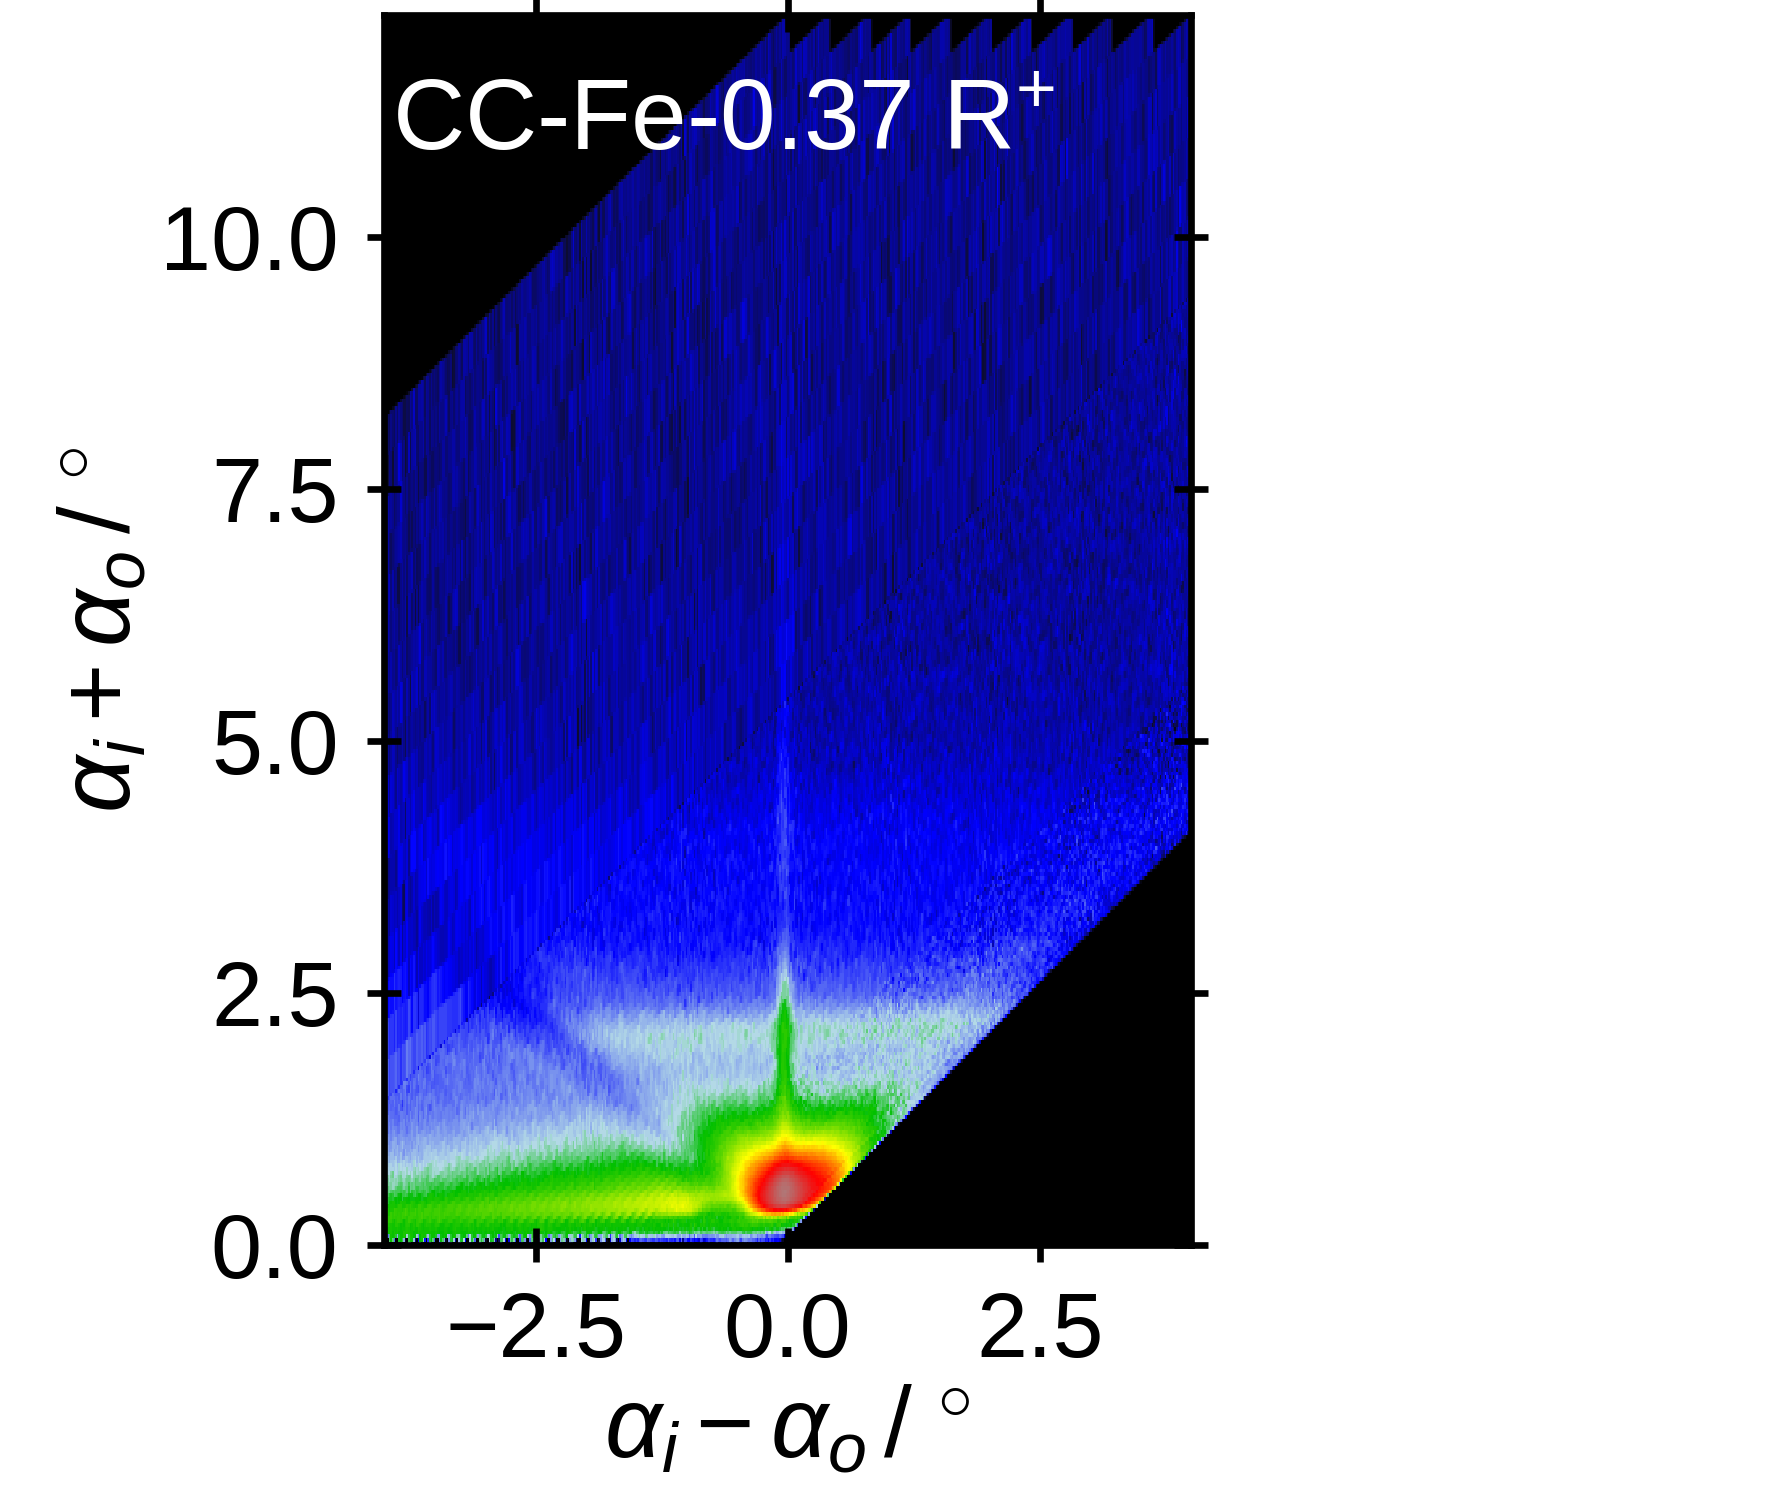
\includegraphics{colloidalCrystals_PNR_CC_Fe_0_37_rem_ud_ReflectivityMapFC}
    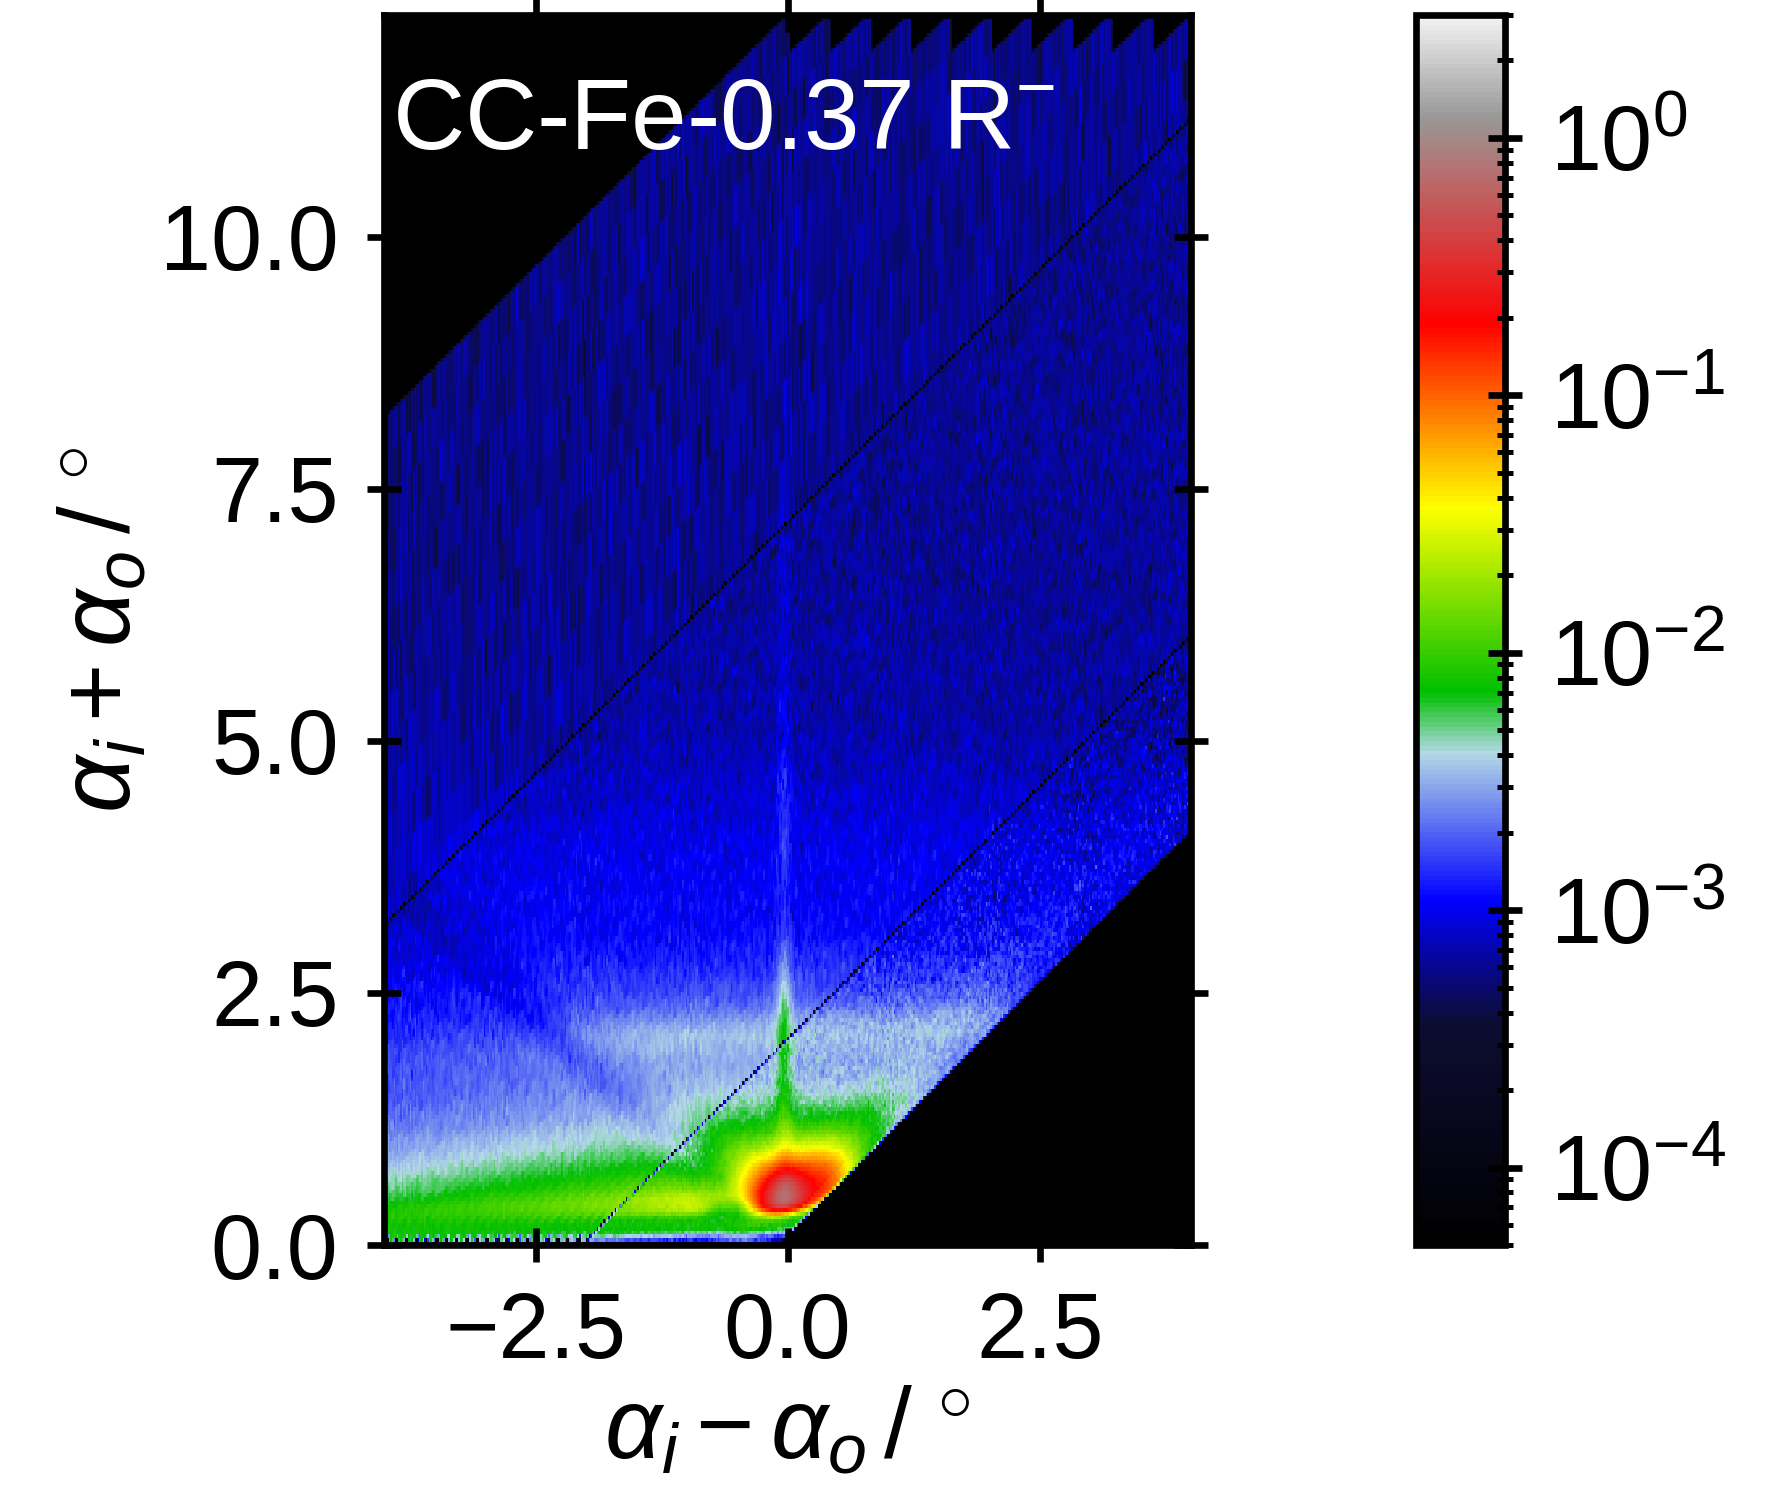
\includegraphics{colloidalCrystals_PNR_CC_Fe_0_37_rem_dd_ReflectivityMapFC}
    \caption{\label{fig:colloidalCrystals:pnrRemanenceMaps} Reflectivitiy maps of CC-Fe-0.37 obtained after field cooling the sample at $1.08 \unit{T}$ to $10 \unit{K}$ and measuring the sample at remanence at the guide field of $0.9 \unit{mT}$. The reflectivity for both channels $R^{+}$ (left) and $R^{-}$ (right) are shown.}
  \end{figure}

  To study the magnetic structure of the colloidal crystals, polarized neutron reflectivity was measured at the MARIA instrument at MLZ (\refsec{ch:lss:maria}).
  For each sample and measurement a reflectivity maps is obtained for $R^{+}$ and $R^{-}$, which is exemplary shown for the measurement obtained in remanence after field-cooling CC-Fe-0.37 to $10 \unit{K}$ at $1.08\unit{T}$ and measuring at the guide field of $0.9 \unit{mT}$ in \reffig{fig:colloidalCrystals:pnrRemanenceMaps}.
  The reflectivity map are similar in nature to the ones obtained for XRR in \refsec{sec:colloidalCrystals:layers:xrr} and all show as main feature the specular line with high intensity and an additional Bragg sheets in the off-specular region around $\alpha_i + \alpha_o \eq 2.2^\circ$.
  In the case of the remanent measurement after field cooling, a difference in intensity is already visible in the reflectivity map, where the reflectivity is more intense in the $R^{+}$ than in the $R^{-}$ case, which follows from the magnetized state of the sample.

  \begin{figure}[tb]
    \centering
    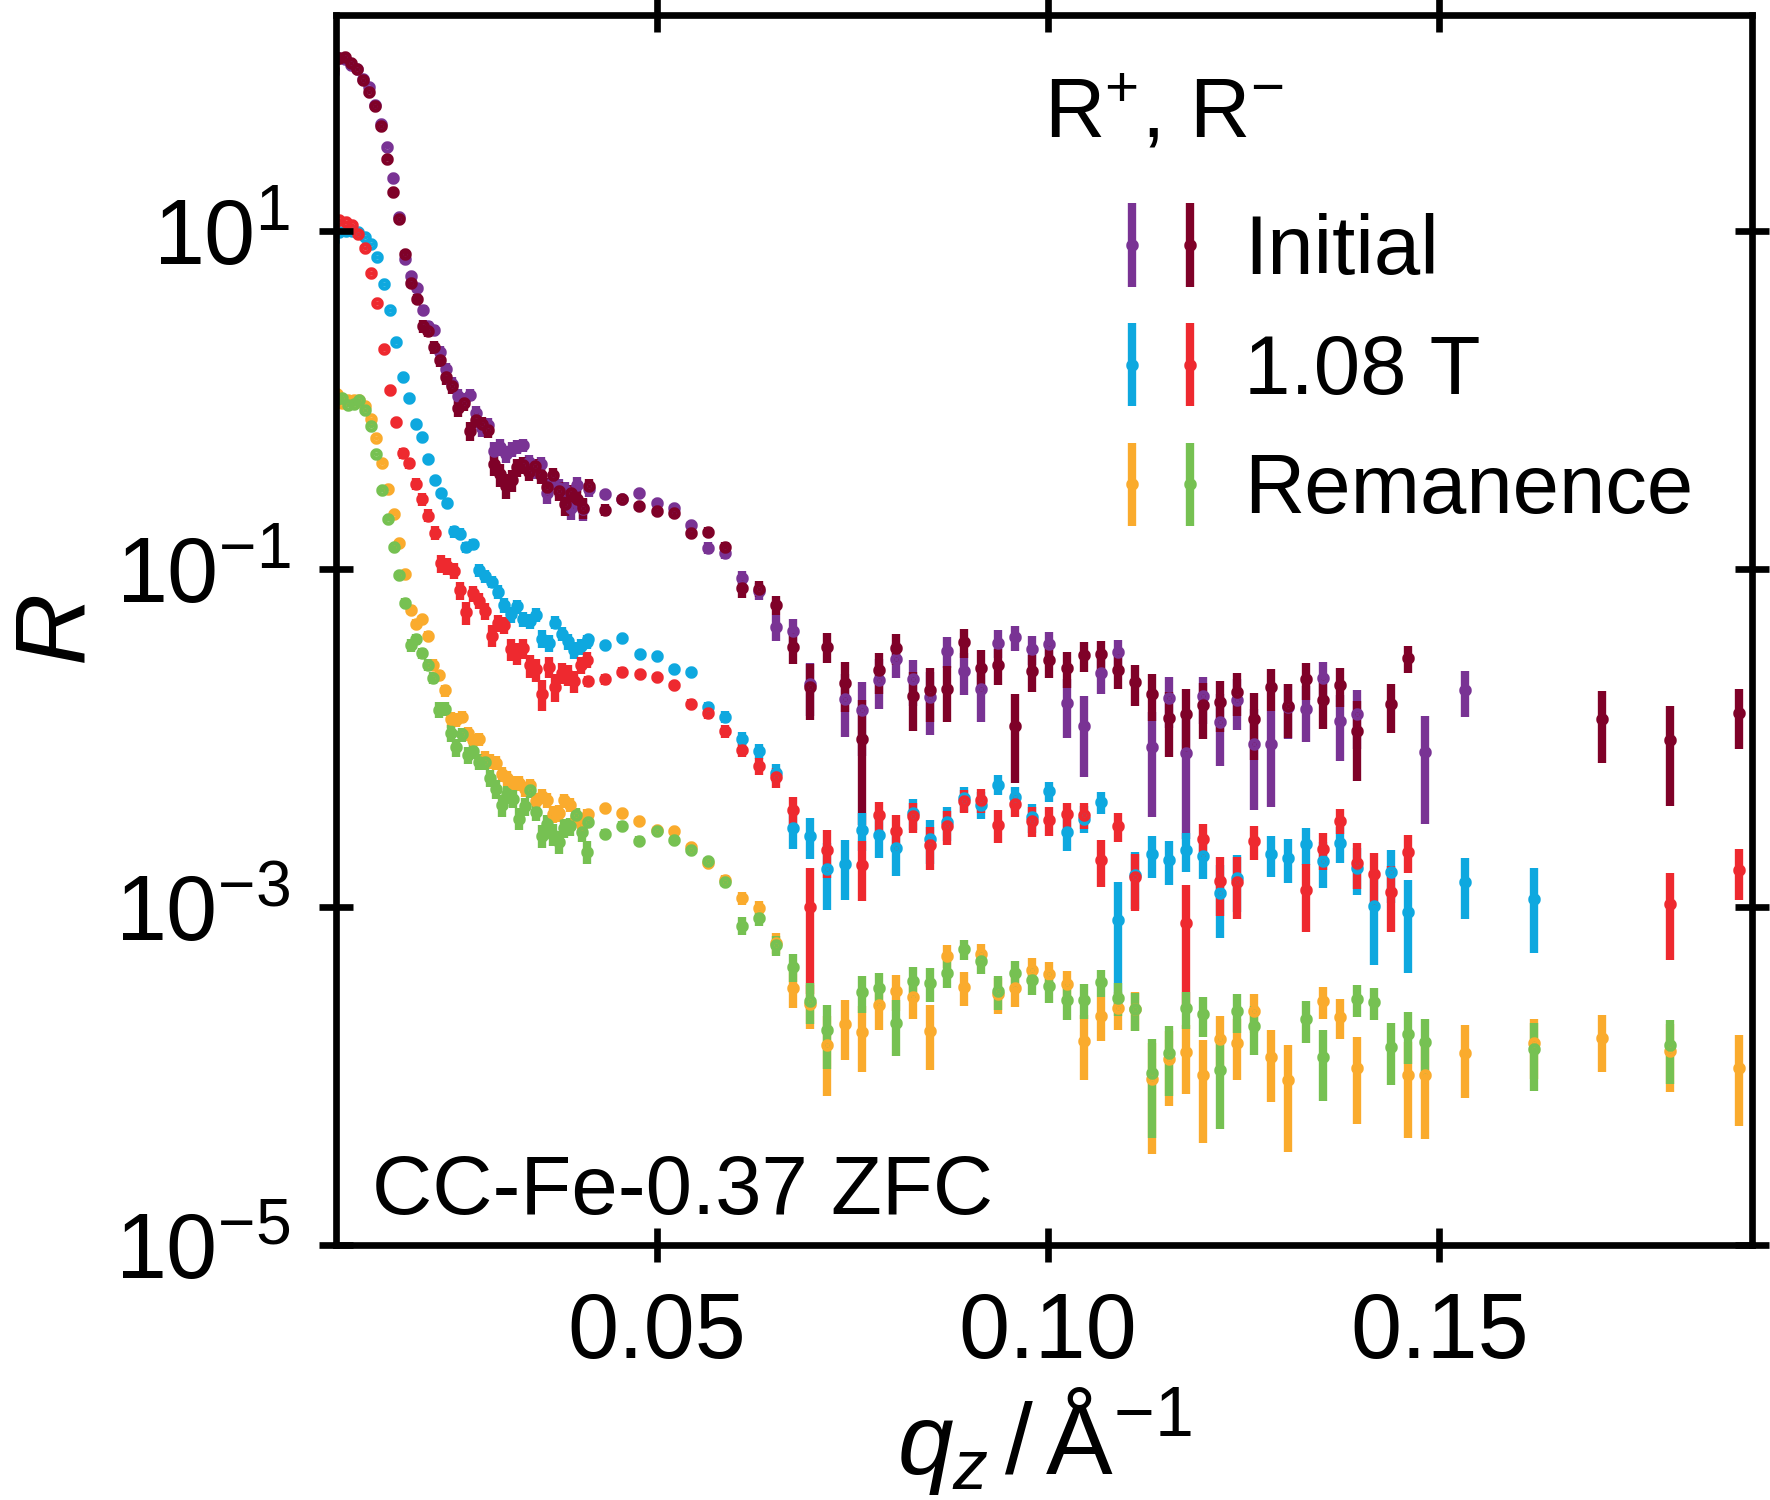
\includegraphics{colloidalCrystals_VerticalStructure_CC-Fe-0_37_PNR_ZFC10K}
    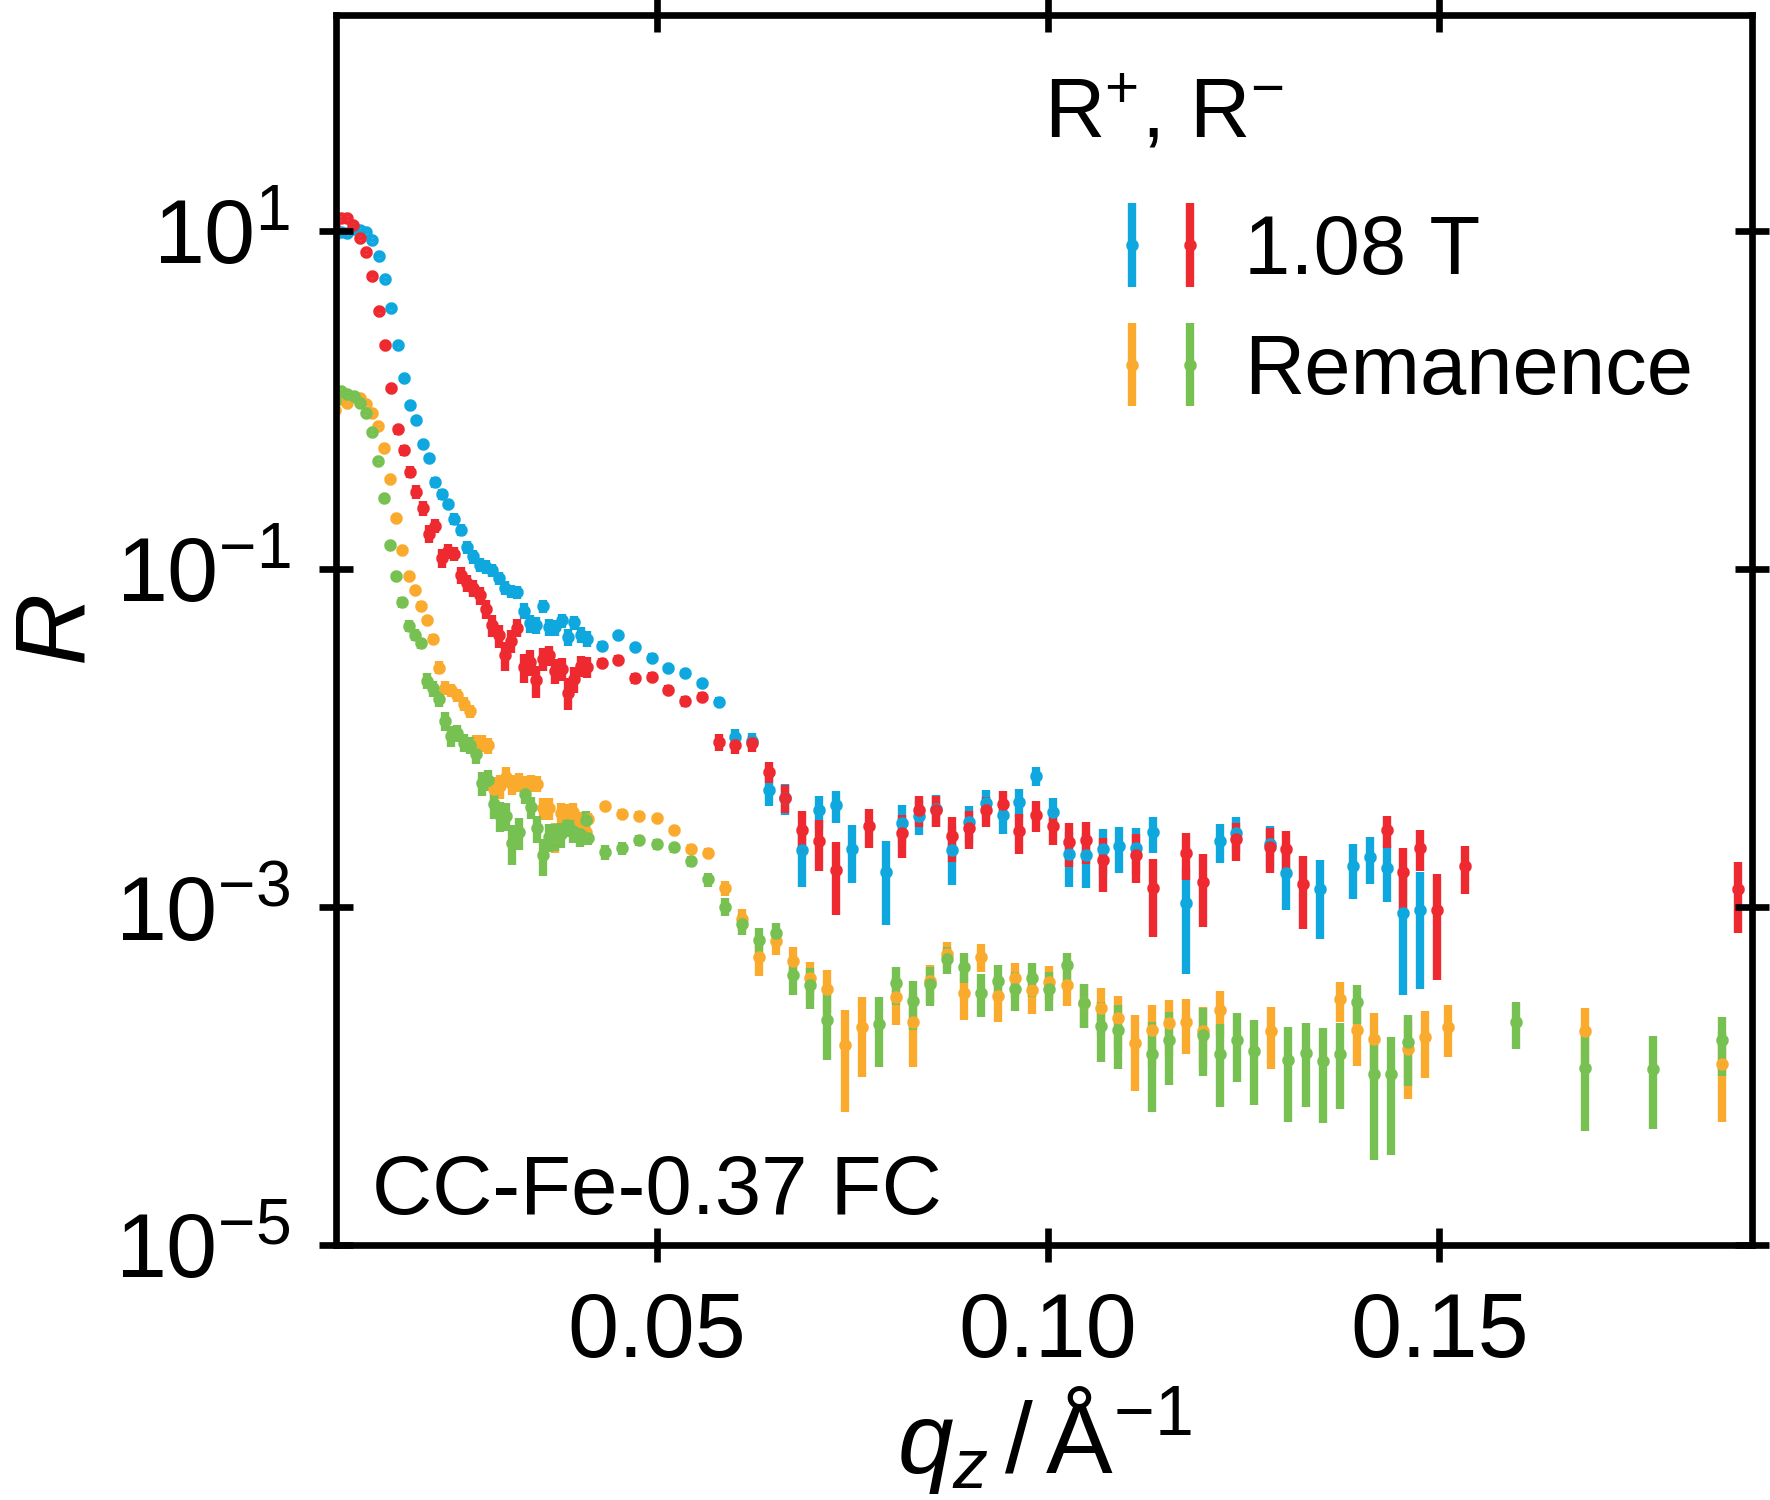
\includegraphics{colloidalCrystals_VerticalStructure_CC-Fe-0_37_PNR_FC10K}
    \caption{\label{fig:colloidalCrystals:pnrCCFe37}Specular reflectivity of CC-Fe-0.37 obtained after zero-field cooling (left) and field cooling (right). The reflectivity is measured at $10 \unit{K}$ with polarized neutrons at varied magnetic states: in the ZFC case initially at guide field, at $1.08 \unit{T}$ and in remanence at guide field again, and for the FC case at high field and in remanence.}
  \end{figure}

  The reduced reflectivities, extracted from each intensity map, are shown for CC-Fe-0.37 in \reffig{fig:colloidalCrystals:pnrCCFe37} for the measurements performed after zero-field cooling and field-cooling.
  In the saturated state both the zero-field cooled and the field cooled measurement show a visible splitting of the two channels due to the magnetization of the sample.
  At remanence, this is still clearly visible for the field cooled case, as was also apparent in the reflectivity map, but is less pronounced in the zero-field cooled reflectivity at remanence.
  The same tendential behaviour is observable in the case of the sample CC-Fe-0.25 and for CC-Fe-0.50 in \reffig{fig:colloidalCrystals:pnrCCFe2550}.

  It is visible in the reflectivity of CC-Fe-0.50 that analogously to it's XRR measurement in \refsec{sec:colloidalCrystals:layers:xrr} the critical edge reduced to a lower scattering angle for this sample in comparison to CC-Fe-0.25 and CC-Fe-0.37.
  Observing this in the case of the X-ray experiment and neutron experiment reinforces that this observation is a feature from the sample and not possibly an artifact from a malfunction during the measurement procedure.
  It is connected to the large thickness of the sample, and suggests a lower average scattering length density in comparison to the silicon layer, as the position of the critical edge is directly proportional to the scattering length density.

  The correlation peak around $0.5 \unit{nm^{-1}}$ and $1 \unit{nm^{-1}}$ in each measurement corresponds with $2 \pi / \Delta q \approx 12.6 \unit{nm}$ to the length scale of the nanocube size.
  Additional features from the layered structure or the total sample thickness, by the means of Kiessig fringes, are not visible within the datasets, which reinforces the assumption that still the samples are rough on the surface.
  A detailed modeling of the scattering length density profile has not been performed within this thesis and might be considered as highly ambiguous due to the low number of features in the reflectivity but the complex three-dimensional structure of the samples.
  An access might be given from the GISAXS analysis of CC-Fe-0.37 in \refsec{sec:colloidalCrystals:layers:gisaxs}, where a $bct$ unit cell was determined from the observed reflections.
  Translating this to a model of the laterally averaged scattering length density along the vertical axis should reproduce the observed features of the reflectivity.

  Qualitatively it is visible that a splitting remains in the remanent state, which is stronger for the field cooled case in direct comparison to the zero-field cooled case.
  This connects to the comparison of the hysteresis curve of the samples after zero-field and field cooling in \refsec{sec:colloidalCrystals:vsm}, where an exchange bias effect is visible that is argued to be a property of the core-shell nanocubes.
  Signatures for emergent dipolar interaction effects from the qualitative comparison of the three samples are not directly observable from the obtained polarized neutron reflectometry data.


  \begin{figure}[tb]
    \centering
    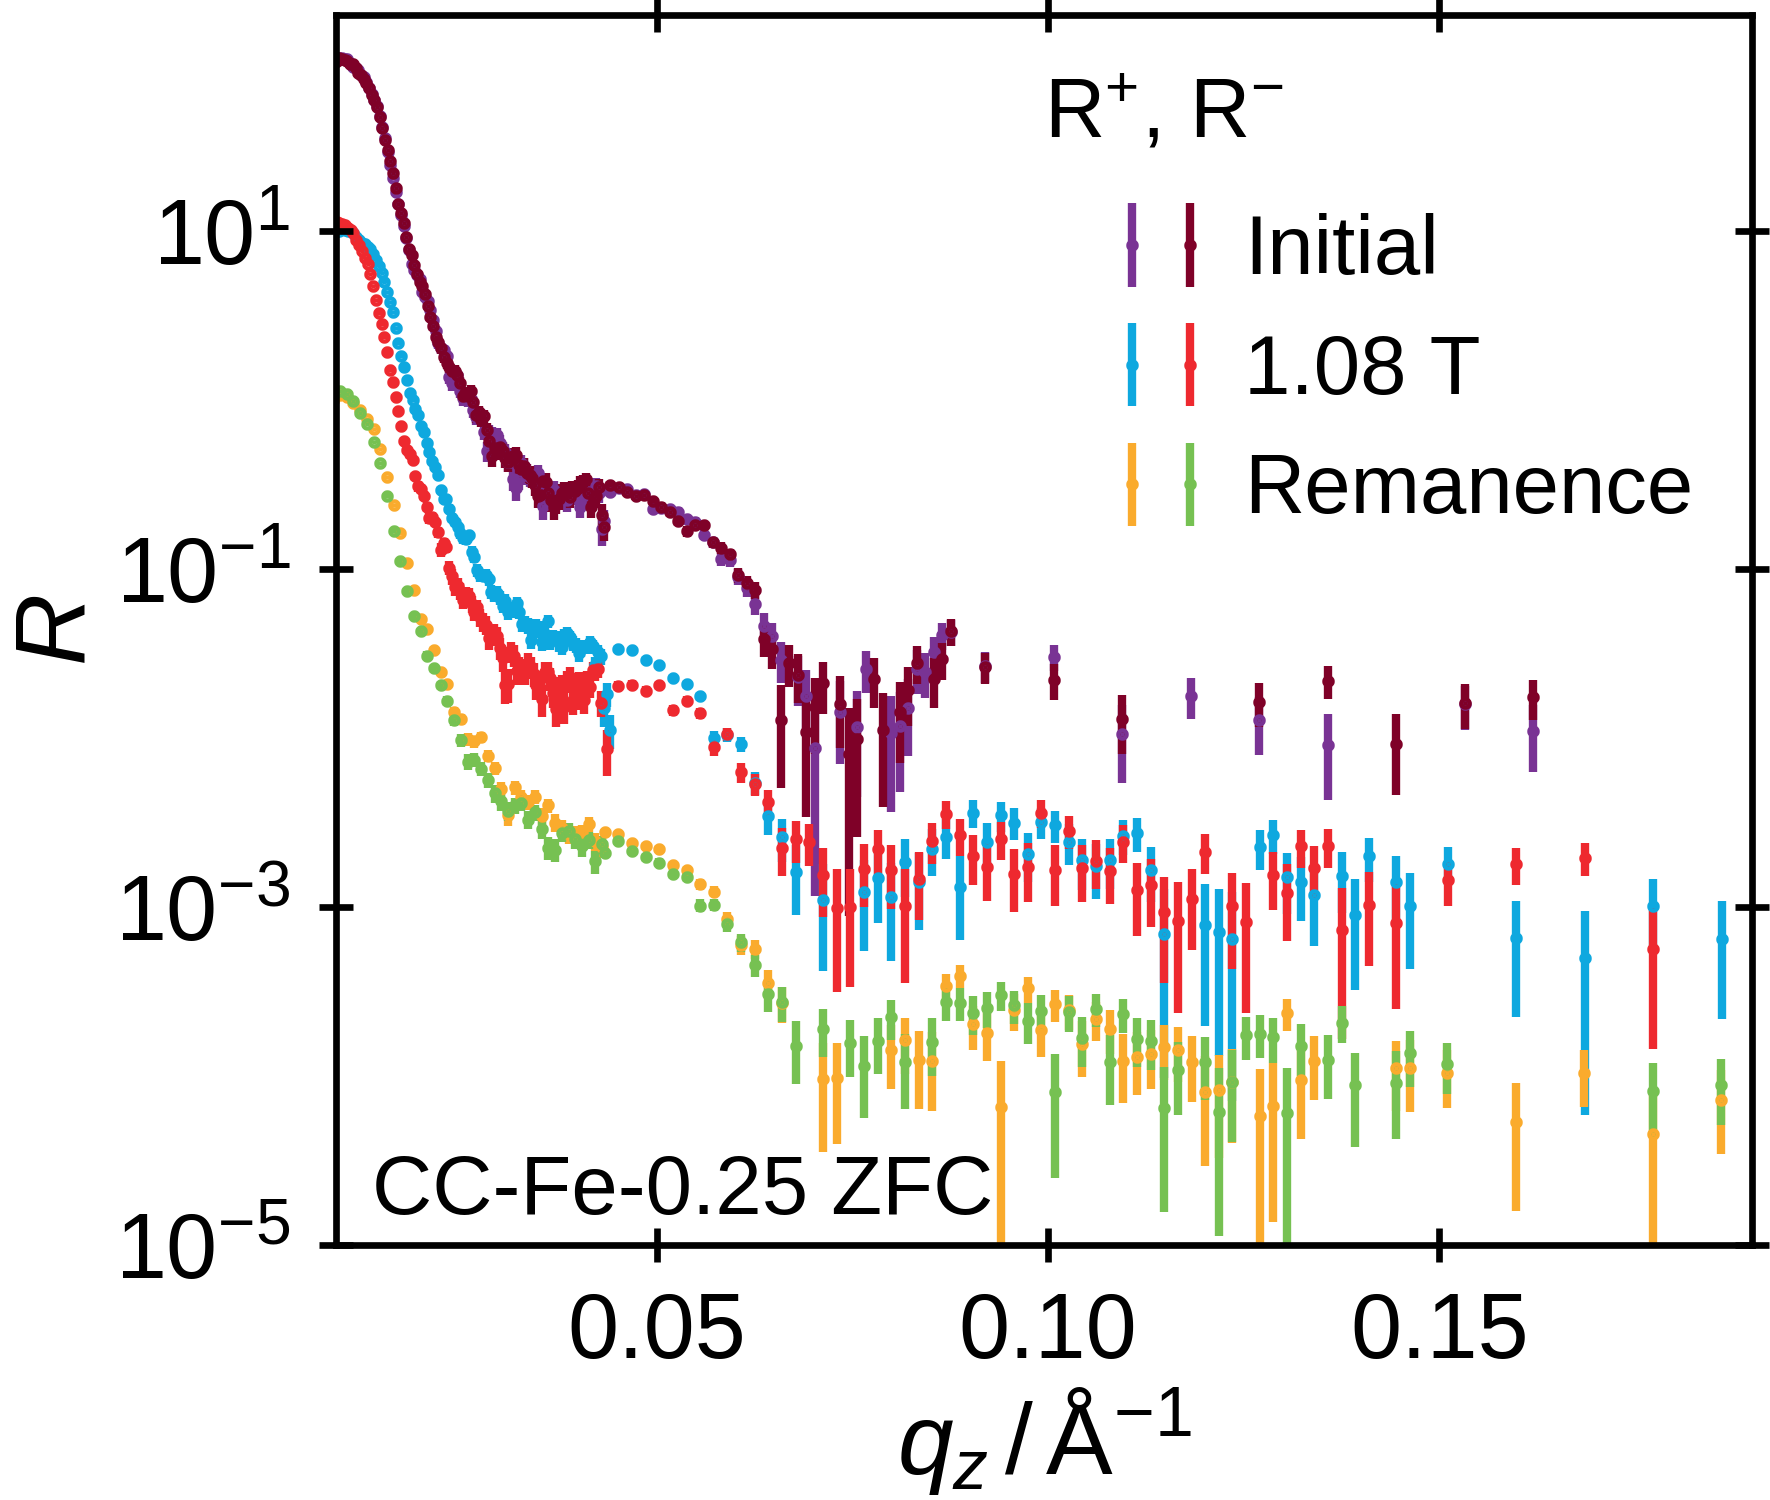
\includegraphics{colloidalCrystals_VerticalStructure_CC-Fe-0_25_PNR_ZFC10K}
    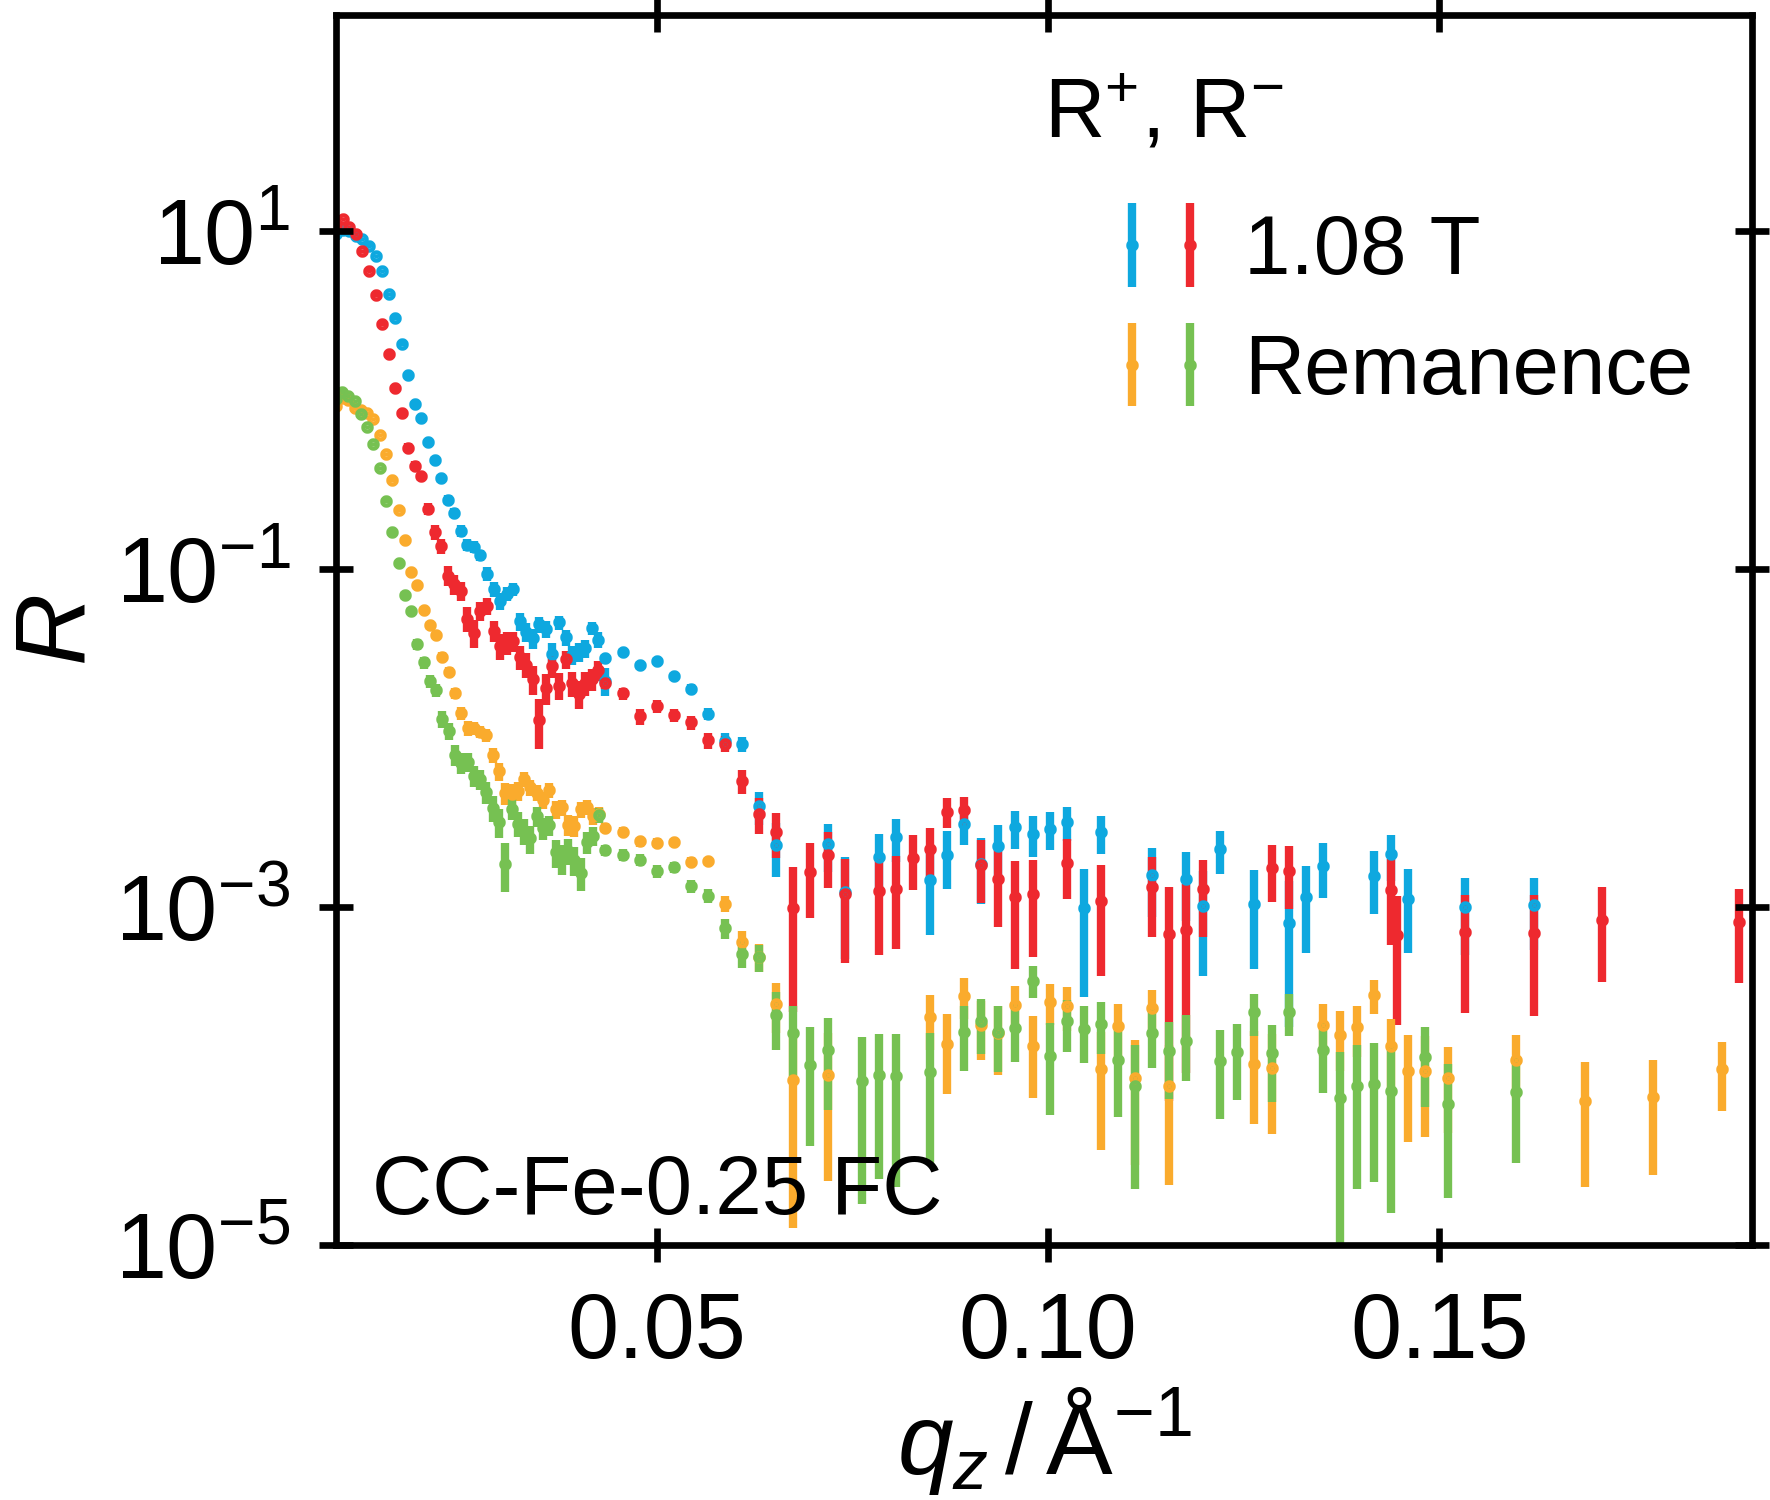
\includegraphics{colloidalCrystals_VerticalStructure_CC-Fe-0_25_PNR_FC10K}
    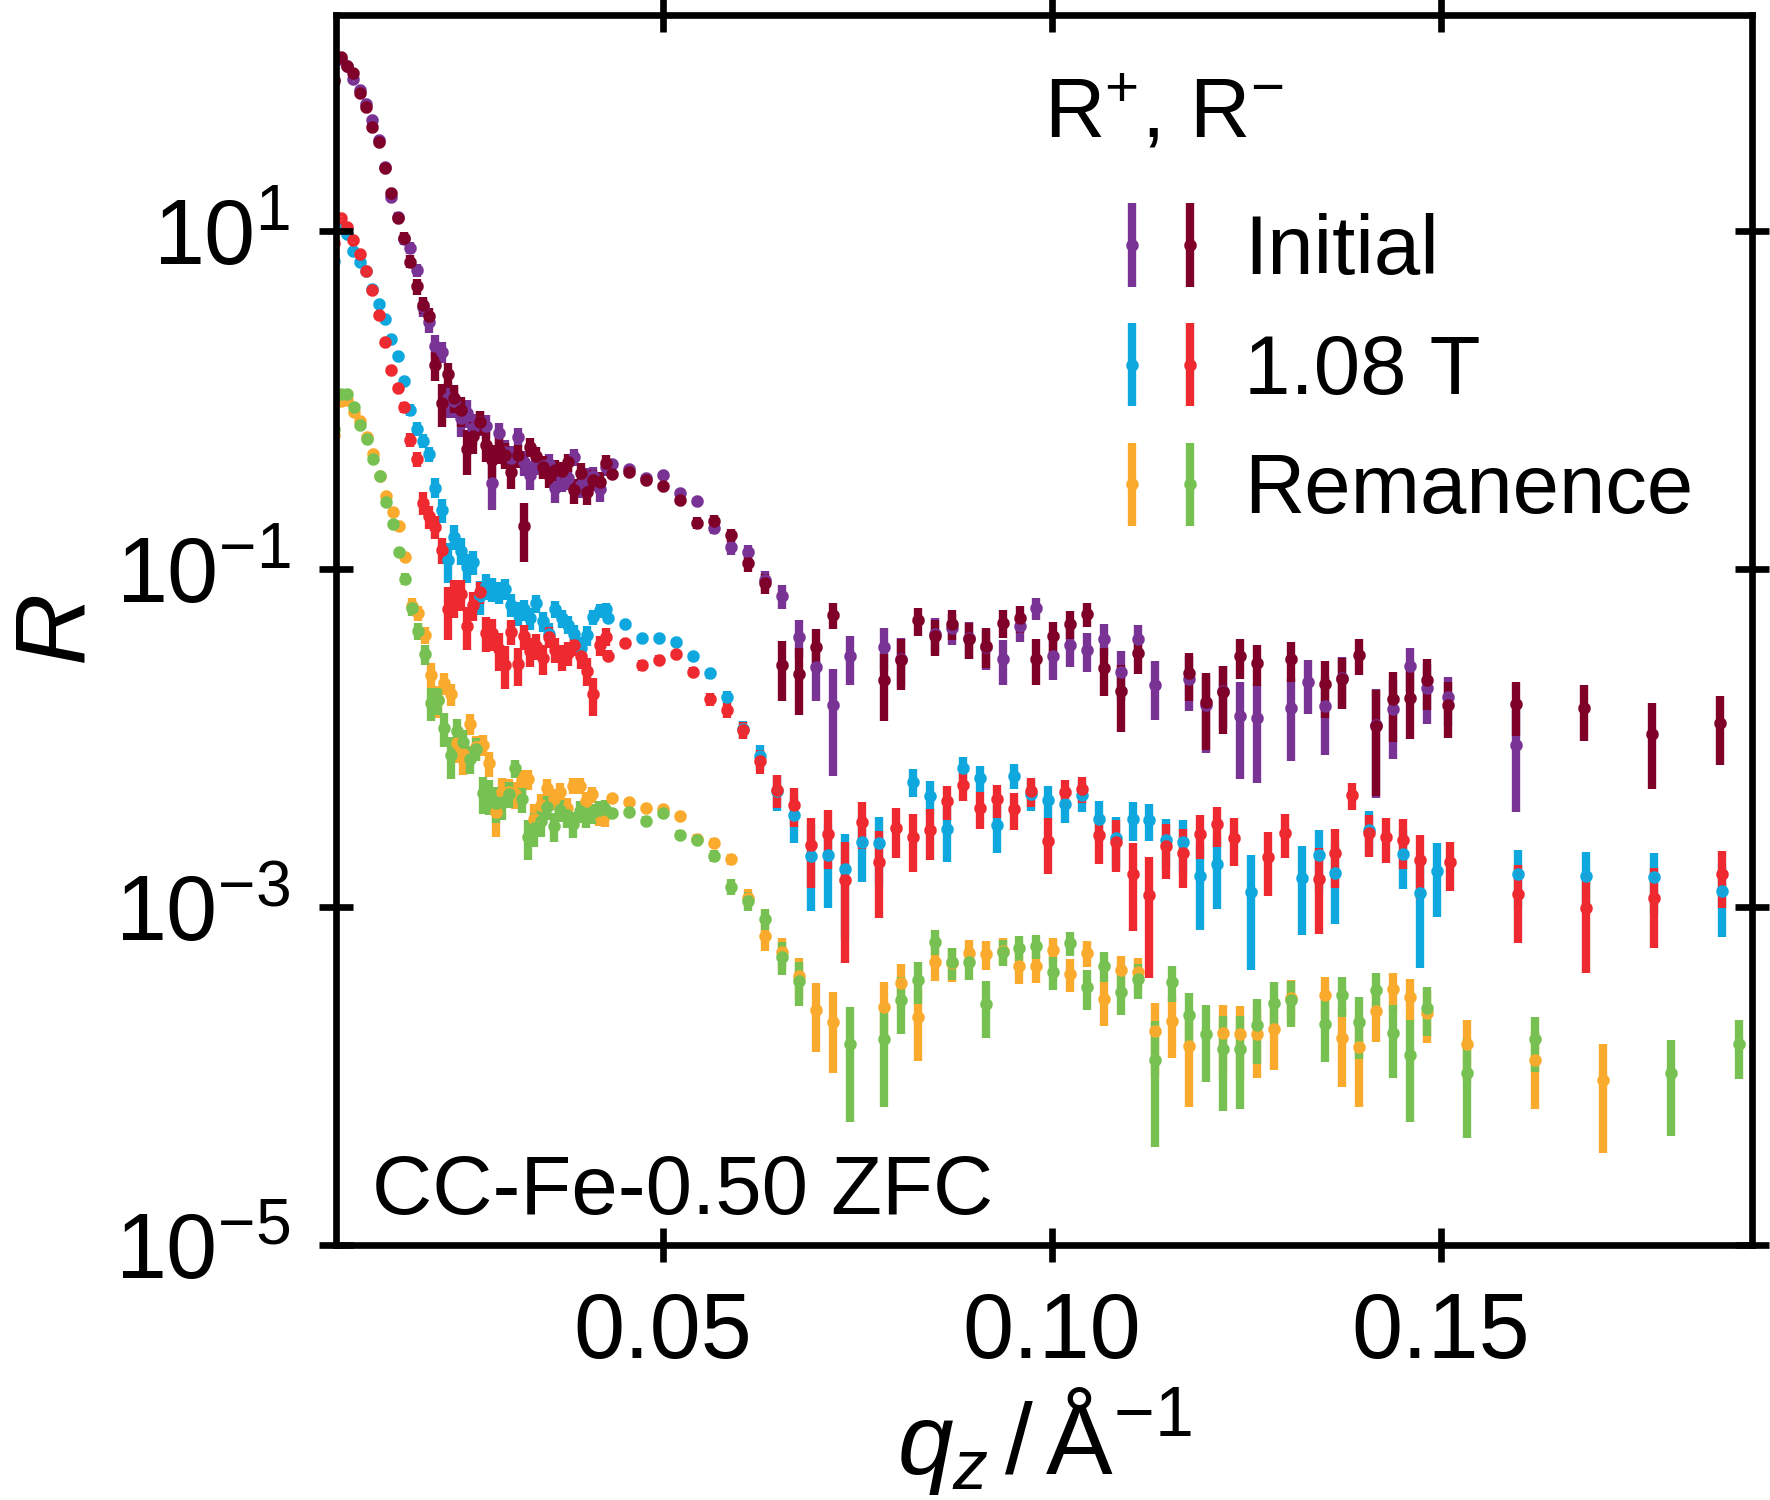
\includegraphics{colloidalCrystals_VerticalStructure_CC-Fe-0_50_PNR_ZFC10K}
    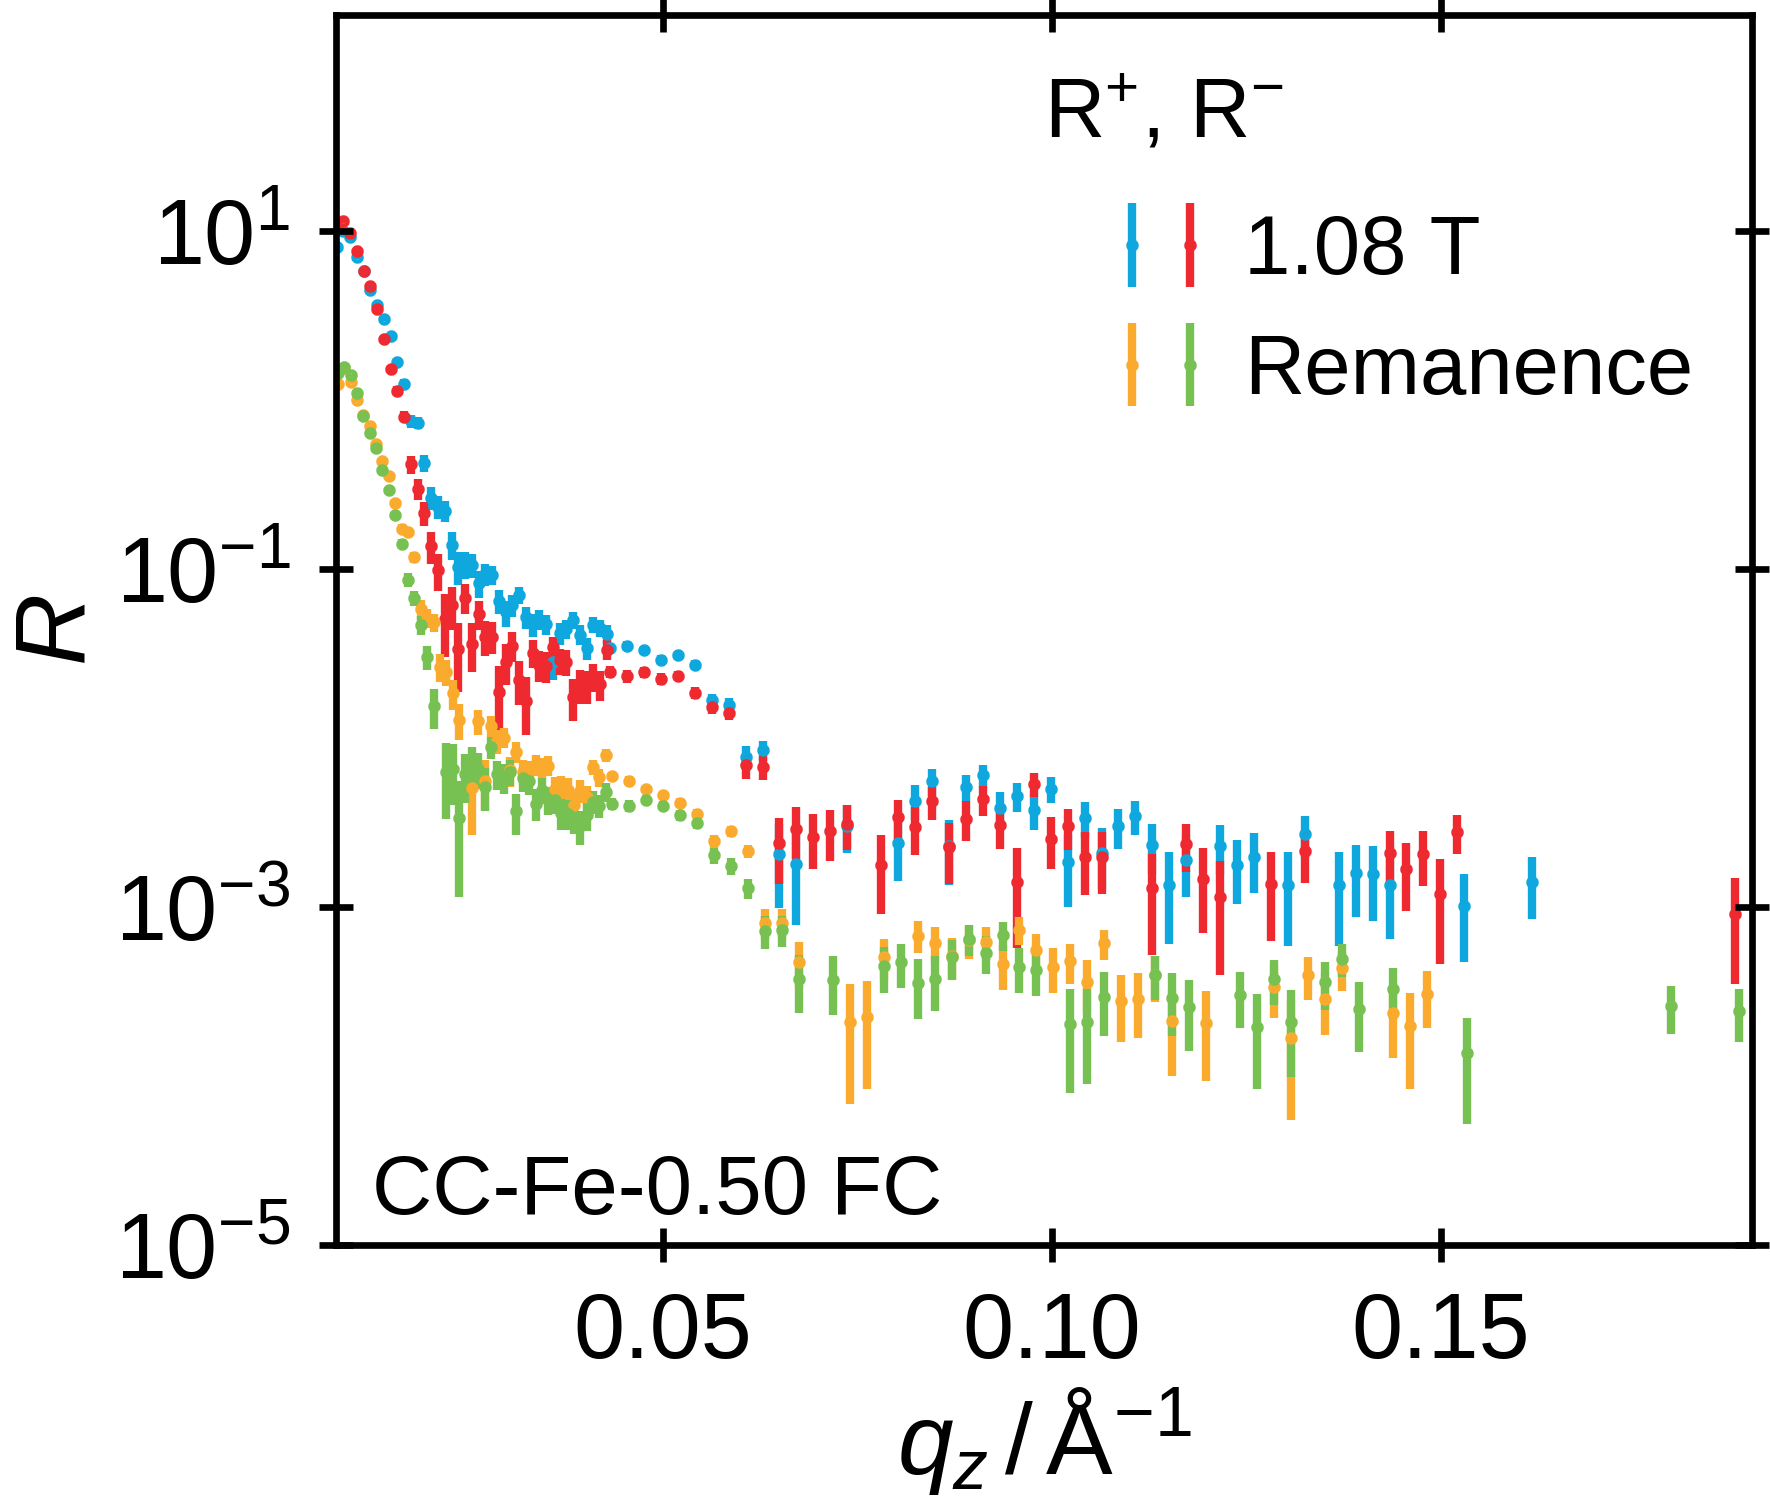
\includegraphics{colloidalCrystals_VerticalStructure_CC-Fe-0_50_PNR_FC10K}
    \caption{\label{fig:colloidalCrystals:pnrCCFe2550} The specular reflectivity of CC-Fe-0.25 (upper) and CC-Fe-0.50 (lower) after zero-field cooling (left) and field cooling (right). The shown measurements are analogue to \reffig{fig:colloidalCrystals:pnrCCFe37}.}
  \end{figure}
\end{document}